% Presentation flag: uncomment to enable presentation features (slower compilation)
\newcommand*{\PRESENTATION}

% Preliminaries
\ifdefined\PRESENTATION
	\documentclass[t]{beamer}
\else
	\documentclass[t,handout]{beamer}
\fi
\mode<presentation>
\usetheme{Warsaw}
\useoutertheme{infolines} 

% Includes
\usepackage{lmodern}
\usepackage{amsmath}
\usepackage{amsfonts}
\usepackage{bbm}
\usepackage{bm}
\usepackage{nicefrac}
\usepackage{color}
\usepackage{perpage}
\usepackage{multicol}
\usepackage{tikz}
\usepackage{tikz-dependency}
\usetikzlibrary{graphs,graphs.standard,graphdrawing,quotes,shapes}
\usegdlibrary{layered}

\makeatletter
\pgfdeclareshape{vector}{
	  \inheritsavedanchors[from={rectangle}]
	  \inheritbackgroundpath[from={rectangle}]
	  \inheritanchorborder[from={rectangle}]
	  \foreach \x in {center,north east,north west,north,south,south east,south west,east,west}{
	    \inheritanchor[from={rectangle}]{\x}
	  }

    \backgroundpath{
      \pgftransformshift{\pgfpoint{-16pt}{-4pt}}
		  \draw[rounded corners=2pt] (0,0) rectangle (32pt,8pt);
    }

    \beforebackgroundpath{
      \draw[step=8pt,help lines,-] (8pt,.1pt) grid (24pt,7.9pt);
    }
}
\makeatother

\MakePerPage{footnote}

% Outline slides
\AtBeginSection
{\begin{frame} \frametitle{Outline} \tableofcontents[currentsection,currentsubsection] \end{frame}}
\AtBeginSubsection
{\begin{frame} \frametitle{Outline} \tableofcontents[currentsection,currentsubsection] \end{frame}}


\begin{document}

\title[]{Universal Semantic Parsing with Neural Networks}
\author{Daniel Hershcovich}
\institute[]{PhD Committee Meeting}
\date{October 25, 2016}

\begin{frame}
\titlepage
\end{frame}


\section{Semantic Annotation Schemes}

\begin{frame}
\frametitle{Semantic Annotation Schemes}
\begin{itemize}
 \item Semantic Role Labeling
 \item Semantic Dependencies
 \item Abstract Meaning Representation
 \item Universal Conceptual Cognitive Annotation
\end{itemize}
\end{frame}

\begin{frame}
\frametitle{Semantic Role Labeling (SRL)}
\centering
\vspace*{\fill}
{\color{blue} PropBank}
\vspace*{\fill}

\begin{dependency}
	\begin{deptext}[column sep=1.5em,ampersand replacement=\^]
	After \^ graduation \^ , \^ John \^ moved \^ to \^ Paris \\
	\end{deptext}
	% PropBank
	\node[xshift=4.91em,yshift=3em,color=blue]{move.01}
	child{node at ($(\wordref{1}{5})$) {}};
	\node[xshift=-9.5em,yshift=3em,color=blue]{AM-TMP}
	child{node at ($(\wordref{1}{1})$) {}}
	child{node at ($(\wordref{1}{2})$) {}};
	\node[xshift=.65em,yshift=3em,color=blue]{A1}
	child{node at ($(\wordref{1}{4})$) {}};
	\node[xshift=10.5em,yshift=3em,color=blue]{A2}
	child{node at ($(\wordref{1}{6})$) {}}
	child{node at ($(\wordref{1}{7})$) {}};
	% FrameNet
	\node[xshift=4.91em,yshift=-3em,color=red]{Motion}
	child{node at ($(\wordref{1}{5})$) {}};
	\node[xshift=-9.5em,yshift=-3em,color=red]{Time}
	child{node at ($(\wordref{1}{1})$) {}}
	child{node at ($(\wordref{1}{2})$) {}};
	\node[xshift=.65em,yshift=-3em,color=red]{Theme}
	child{node at ($(\wordref{1}{4})$) {}};
	\node[xshift=10.5em,yshift=-3em,color=red]{Goal}
	child{node at ($(\wordref{1}{6})$) {}}
	child{node at ($(\wordref{1}{7})$) {}};
\end{dependency}

\vspace*{\fill}
{\color{red} FrameNet}
\end{frame}

\begin{frame}
\frametitle{Semantic Dependency Parsing (SDP)}
\centering
\vspace*{\fill}
{\color{blue} DELPH-IN MRS-derived bi-lexical dependencies (DM)}
\vspace*{\fill}

\begin{dependency}[theme=simple]
	\begin{deptext}[column sep=1.5em,ampersand replacement=\^]
	After \^ graduation \^ , \^ John \^ moved \^ to \^ Paris \\
	\end{deptext}
	\deproot{5}{\color{blue} top}
	\depedge{1}{2}{\color{blue} ARG2}
	\depedge{1}{5}{\color{blue} ARG1}
	\depedge{5}{4}{\color{blue} ARG1}
	\depedge{6}{5}{\color{blue} ARG1}
	\depedge{6}{7}{\color{blue} ARG2}
	\deproot[edge below]{5}{\color{red} top}
	\depedge[edge below]{5}{2}{\color{red} TWHEN}
	\depedge[edge below]{5}{4}{\color{red} ACT-arg}
	\depedge[edge below]{5}{7}{\color{red} DIR3-arg}
\end{dependency}

\vspace*{\fill}
{\color{red} Prague Dependency Treebank tectogrammatical layer (PSD)}
\end{frame}

\begin{frame}
\frametitle{Abstract Meaning Representation (AMR)}
\begin{tikzpicture}
\graph[layered layout, sibling distance=5cm, layer distance=2cm, edges={nodes={sloped}}]{
a4 Paris[as={Paris}, black];
a2 John[as={John}, black];
a1[as={person}, black];
a0[as={move-01}, black];
a3[as={city}, black];
a2[as={name}, black];
a5[as={after}, black];
a4[as={name}, black];
a6[as={graduate-01}, black];

a1 ->  ["name"' above, black] a2;
a0 ->  ["ARG0"' above, black] a1;
a0 ->  ["ARG2"' above, black] a3;
a0 ->  ["time"' above, black] a5;
a3 ->  ["name"' above, black] a4;
a2 ->  ["op1"' above, black] a2 John;
a5 ->  ["op1"' above, black] a6;
a4 ->  ["op1"' above, black] a4 Paris;
};
\draw[->, above, black] (a6) to node[sloped] {ARG0} (a1);
\end{tikzpicture}
\end{frame}

\begin{frame}
\frametitle{Universal Conceptual Cognitive Annotation (UCCA)}
\centering
\vspace*{\fill}
\begin{tikzpicture}[level distance=2cm, sibling distance=25mm, ->]
    \node (ROOT) [fill=black, circle] {}
      child {node (After) {After} edge from parent node[left] {\scriptsize $L$\;}}
      child {node (graduation) [fill=black, circle] {}
      {
        child {node {graduation} edge from parent node[left] {\scriptsize $P$}}
      } edge from parent node[left] {\scriptsize $H$} }
      child {node {,} edge from parent node[right] {\scriptsize $U$}}
      child {node (moved) [fill=black, circle] {}
      {
        child {node (John) {John} edge from parent node[left] {\scriptsize $A$}}
        child {node {moved} edge from parent node[left] {\scriptsize $P$}}
        child {node [fill=black, circle] {}
        {
          child {node {to} edge from parent node[left] {\scriptsize $R$}}
          child {node {Paris} edge from parent node[left] {\scriptsize $C$}}
        } edge from parent node[left] {\scriptsize $A$} }
      } edge from parent node[right] {\scriptsize $H$} }
      ;
    \draw[dashed,->] (graduation) to node [auto] {\scriptsize $A$} (John);
    \node (LKG) at (-1.8,0) [fill=black!20, circle] {};
        \draw[bend right] (LKG) to node [auto, left] {\scriptsize $LR$} (After);
        \draw (LKG) to[out=-60, in=120] node [below] {\scriptsize $LA$\quad\;} (graduation);
        \draw (LKG) to[out=30, in=90] node [above] {\scriptsize $LA$} (moved);
\end{tikzpicture}
\vspace*{\fill}
\end{frame}

\begin{frame}
\frametitle{Structural Properties}
\noindent
(1) non-terminal nodes, (2) reentrancy, (3) discontinuity
\centering
\vspace*{\fill}
\begin{minipage}{.48\linewidth}{\centering
  \begin{tikzpicture}[level distance=12mm, sibling distance=16mm, ->,
      every node/.append style={midway}]
    \node (ROOT) [fill=black, circle] {}
      child {node [fill=black, circle] {}
      {
        child {node {John} edge from parent node[left] {\scriptsize $C$}}
        child {node {and} edge from parent node[left] {\scriptsize $N$}}
        child {node {Mary} edge from parent node[left] {\scriptsize $C$}}
      } edge from parent node[left] {\scriptsize $A$} }
      child {node {went} edge from parent node[left] {\scriptsize $P$}}
      child {node {home} edge from parent node[left] {\scriptsize $A$}}
      ;
  \end{tikzpicture}
  }
\end{minipage}
\hfill
\begin{minipage}{.48\linewidth}{\centering
  \begin{tikzpicture}[level distance=12mm, sibling distance=2cm, ->,
      every node/.append style={midway}]
    \node (ROOT) [fill=black, circle] {}
      child {node {John} edge from parent node[left] {\scriptsize $A$}}
      child {node [fill=black, circle] {}
      {
      	child {node {gave} edge from parent node[left] {\scriptsize $C$}}
      	child {node (everything) {everything} edge from parent[white]}
      	child {node {up} edge from parent node[left] {\scriptsize $C$}}
      } edge from parent node[right] {\scriptsize $P$} }
      ;
    \draw[bend right,->] (ROOT) to[out=-20, in=180] node [left] {\scriptsize $A$} (everything);
  \end{tikzpicture}
  }
\end{minipage}

\vspace{-6mm}
  \begin{tikzpicture}[level distance=12mm, sibling distance=2cm, ->,
      every node/.append style={midway}]
    \node (ROOT) [fill=black, circle] {}
      child {node (John) {John} edge from parent node[left] {\scriptsize $A$}}
      child {node {decided} edge from parent node[left] {\scriptsize $P$}}
      child {node (totakeaquickshower) [fill=black, circle] {}
      {
        child {node {to} edge from parent node[left] {\scriptsize $F$}}
        child {node (takeashower) [fill=black, circle] {}
        {
          child {node {take} edge from parent node[left] {\scriptsize $C$}}
          child {node {a} edge from parent node[right] {\scriptsize $F$}}
          child {node (quick) {quick} edge from parent[white]}
          child {node {shower} edge from parent node[right] {\scriptsize $C$}}
        } edge from parent node[right] {\scriptsize $P$} }
      } edge from parent node[left] {\scriptsize $A$} }
      ;
    \draw[bend left,dashed,->] (takeashower) to node [auto] {\scriptsize $A$} (John);
    \draw[bend left,->] (totakeaquickshower) to node [auto] {\scriptsize $D$} (quick);
  \end{tikzpicture}
\end{frame}


\begin{frame}
\frametitle{UCCA Corpora}
\begin{center}
	\begin{tabular}{l|ccc|c}
	& \multicolumn{3}{c|}{Wiki} & 20K \\
	& \small Train & \small Dev & \small Test & Leagues \\
	\hline
	\# passages & 300 & 34 & 34 & 154 \\
	\# sentences & 4267 & 453 & 518 & 506 \\
	\hline
	\# nodes & 298,665 & 33,263 & 37,262 & 29,315 \\
	\% terminal & 42.95 & 43.62 & 42.89 & 42.09 \\
	\% non-term. & 58.30 & 57.46 & 58.31 & 60.01 \\
	\% discont. & 0.53 & 0.51 & 0.47 & 0.81 \\
	\% reentrant & 2.31 & 1.76 & 2.18 & 2.03 \\
	\hline
	\# edges & 287,381 & 32,015 & 35,846 & 27,749 \\
	\% primary & 98.29 & 98.81 & 98.75 & 97.73 \\
	\% remote & 1.71 & 1.19 & 1.25 & 2.27 \\
	\hline
	\multicolumn{3}{l}{\footnotesize Average per non-terminal node} \\
	\# children & 1.67 & 1.68 & 1.66 & 1.61 
	\end{tabular}
\end{center}

Excluding root node, implicit nodes, and linkage nodes and edges.
\end{frame}


\section[]{UCCA Parsing}

\begin{frame}
\frametitle{Goal 1: UCCA Parser}
Fast and accurate parser supporting UCCA's structural properties.

\vspace*{\fill}
Impact:
\begin{itemize}
\item New general techniques for broad-coverage parsing.
\item Meaning representation for machine translation and its evaluation.\footnote{
Alexandra Birch, Barry Haddow, Ond\v{r}ej Bojar, and Omri Abend. 2016. HUME: Human UCCA-based
evaluation of machine translation. arXiv preprint arXiv:1607.00030}
\item Semantic features for text understanding based on the graph.

\vspace*{\fill}
\end{itemize}
\begin{center}
 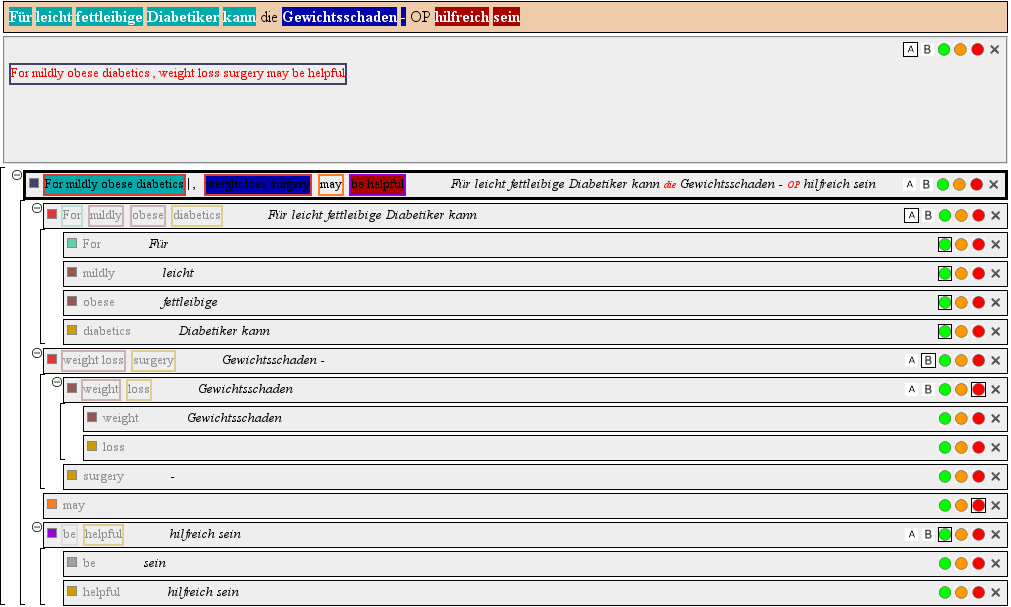
\includegraphics[width=0.6\textwidth,keepaspectratio]{hume}
\end{center}
\end{frame}

\begin{frame}
\frametitle{Transition-Based Parsing}
Parse sentence $w_1 \ldots w_n$ to graph $G=(V,E,\ell)$ incrementally, using buffer $B$ and stack $S$.
Classifier determines transition to apply at each step.

\vspace*{\fill}
\pause
\begin{center}
	\begin{tikzpicture}
	\draw[xstep=2cm,ystep=0.5cm,color=gray] (-.01,0) grid (4,.5);
	\node[anchor=west] at (-.5,.25) {$\bm S$};
	\node[anchor=west] at (0,.25) {After};
	\node[anchor=west] at (2,.25) {graduation};
	\draw[xstep=1.5cm,ystep=0.5cm,color=gray] (4.49,0) grid (10.5,.5);
	\node[anchor=west] at (4,.25) {$\bm B$};
	\node[anchor=west] at (4.5,.25) {John};
	\node[anchor=west] at (6,.25) {moved};
	\node[anchor=west] at (7.5,.25) {to};
	\node[anchor=west] at (9,.25) {Paris};
	\node[anchor=west] at (3,-.5) {$\bm G$};
	\node (ROOT) [fill=black, circle] at (5,-.5) {}
	  child {node  {After} edge from parent [->] node[left] {\scriptsize $L$\;}}
	  child {node [fill=black, circle] {}
	  {
	    child {node {graduation} edge from parent [->] node[right] {\scriptsize $P$}}
	  } edge from parent [->] node[right] {\scriptsize $H$} };
	\end{tikzpicture}
\end{center}

\vspace*{\fill}
\pause
Transitions for UCCA parsing:\\
\textsc{Shift, Reduce, Node$_X$,}\\
\textsc{Left-Edge$_X$, Right-Edge$_X$, Left-Remote$_X$, Right-Remote$_X$,}
\textsc{Swap, Finish}\\
\end{frame}


\section[]{Distributed Representation}

\begin{frame}
\frametitle{Goal 2: UCCA-Based Distributed Representation}
Vector representation for sentences and documents,
based on recursive composition on the UCCA graph.

\vspace*{\fill}
Impact:
\begin{itemize}
\item General automatic semantic feature extractor for text.
\item Accurate measure for text similarity.
\item Understand the semantic contribution of different elements.
\end{itemize}

\vspace*{\fill}
\begin{center}
  \begin{tikzpicture}[level distance=1cm, sibling distance=2cm, ->]
    \node (ROOT) [fill=black, vector] {}
      child {node (After) {After} edge from parent [shorten <=3mm]
        node[left] {\scriptsize $L$\;}}
      child {node (graduation) [fill=black, vector] {}
      {
        child {node {graduation} edge from parent node[left] {\scriptsize $P$}}
      } edge from parent node[left] {\scriptsize $H$} }
      child {node {,} edge from parent node[right] {\scriptsize $U$}}
      child {node (moved) [fill=black, vector] {}
      {
        child {node (John) {John} edge from parent [shorten <=2mm]
          node[left] {\scriptsize $A$}}
        child {node {moved} edge from parent node[left] {\scriptsize $P$}}
        child {node [fill=black, vector] {}
        {
          child {node {to} edge from parent node[left] {\scriptsize $R$}}
          child {node {Paris} edge from parent node[left] {\scriptsize $C$}}
        } edge from parent [shorten <=2.5mm,shorten >=3mm] node[left] {\scriptsize $A$} }
      } edge from parent [shorten <=3.5mm,shorten >=4mm] node[right] {\scriptsize $H$} }
      ;
    \draw[dashed,->,shorten <=2.5mm] (graduation) to node [auto] {\scriptsize $A$} (John);
    \node (LKG) at (-1.8,0) [fill=black!20, vector] {};
        \draw[bend right,shorten <=4mm] (LKG) to
          node [auto, left] {\scriptsize $LR$} (After);
        \draw (LKG) to[out=-60, in=120]
          node [below] {\scriptsize $LA$\quad\;} (graduation);
        \draw[shorten <=2mm] (LKG) to[out=30, in=90]
          node [above] {\scriptsize $LA$} (moved);
  \end{tikzpicture}
\end{center}
\end{frame}

\begin{frame}
\frametitle{Recursive Neural Networks}
Word embeddings represent words as vectors in $\mathbb{R}^n$.

\vspace*{\fill}
\pause
Recurrent neural networks (or variations, e.g. LSTM)
represent a sequence based on the vectors for individual elements:

\vspace*{\fill}
\begin{center}
	\begin{tikzpicture}[shorten >=1pt,->]
	\tikzstyle{vertex}=[vector,draw=black]
	\foreach \name/\x in {John/1, and/3, Mary/5, Went/7, Home/9}{
	  \node[vertex] (G-\name) at (\x,1) {};
	  \node (\name) at (\x,0) {\name};
	  \draw (\name) -- (G-\name);
	}
	\foreach \from/\to in {John/and,and/Mary,Mary/Went,Went/Home}
	  \draw [shorten <=5mm,shorten >=5mm] (G-\from) -- (G-\to);
	\end{tikzpicture}
\end{center}

\pause
Recursive neural networks (AKA "tree RNNs", but any DAG works)
use hierarchical structure of the input:

\vspace*{\fill}
\begin{center}
	\begin{tikzpicture}[<-]
	\tikzstyle{vertex}=[vector]
	\node[vertex] {}
	  child {node [vertex] {}
	  {
	    child {node {John} edge from parent node[] {}}
	    child {node {and} edge from parent node[] {}}
	    child {node {Mary} edge from parent node[] {}}
	  } edge from parent node[] {}}
	  child {node {went} edge from parent node[] {}}
	  child {node {home} edge from parent node[] {}}
	  ;
	\end{tikzpicture}
\end{center}
\end{frame}


\section[]{Applications}

\begin{frame}
\frametitle{Goal 3: Applications}
Use the UCCA parser and distributed representation to improve
performance on semantic tasks:
\begin{itemize}
\item Sentiment analysis.
\item Machine translation.
\item Automatic summarization.
\end{itemize}
\end{frame}


\section[]{Experiments}

\begin{frame}
\frametitle{UCCA Parser Experiment}
\begin{itemize}
 \item Transition-based parser using
 \begin{itemize}
   \item Sparse perceptron with binary features.
   \item Dense perceptron with pre-trained word embeddings.
   \item Feedforward neural network with real-valued features.
 \end{itemize}
 \item Baselines: bilexical DAG parsers after conversion.
\end{itemize}
\vspace*{\fill}
\begin{center}
	\begin{dependency}[theme = simple]
	\begin{deptext}[column sep=.7em,ampersand replacement=\^]
	After \^ graduation \^ , \^ John \^ moved \^ to \^ Paris \\
	\end{deptext}
	\depedge{2}{1}{L}
	\depedge{2}{3}{U}
	\depedge[dashed]{2}{4}{A}
	\depedge{5}{4}{A}
	\depedge{2}{5}{H}
	\depedge{7}{6}{R}
	\depedge{5}{7}{A}
	\end{dependency}
	\begin{dependency}[theme = simple]
	\begin{deptext}[column sep=.7em,ampersand replacement=\^]
	John \^ gave \^ everything \^ up \\
	\end{deptext}
	\depedge{1}{2}{A}
	\depedge{3}{2}{A}
	\depedge{4}{2}{C}
	\end{dependency}
  \hspace*{\fill}
	\begin{dependency}[theme = simple]
	\begin{deptext}[column sep=.7em,ampersand replacement=\^]
	John \^ and \^ Mary \^ went \^ home \\
	\end{deptext}
	\depedge[edge start x offset=-6pt]{1}{4}{A}
	\depedge{2}{1}{N}
	\depedge{3}{1}{C}
	\depedge{5}{4}{A}
	\end{dependency}
\end{center}
\end{frame}

\begin{frame}
\frametitle{Results}
\begin{center}
	\begin{tabular}{l|ccc|ccc}
	& \multicolumn{3}{c|}{Primary} & \multicolumn{3}{c}{Remote} \\
	& \textbf{LP} & \textbf{LR} & \textbf{LF} & \textbf{LP} & \textbf{LR} & \textbf{LF} \\
	\hline
	\multicolumn{4}{l}{\rule{0pt}{2ex} \footnotesize Bilexical Approximation} \\
	Upper Bound % on the test set and ood set only
	& 93.4 & 83.7 & 88.3 & 73.9 & 49.5 & 59.3 \vspace{.1cm} \\
	DAGParser
	& 63.7 & 	56.1	 & 59.5	 & 0.8	 & 9.5	 &  1.4 \\
	TurboParser
	& 60.2	 & 47.4	 & 52.9	 & 2.2	 & 7.8	 &  3.4 \\
	\hline
	\multicolumn{4}{l}{\rule{0pt}{2ex} \footnotesize Direct Approach} \\
	Sparse perceptron
	& 64 & 55.6 & 59.5 & 16 & 11.6 & 13.4 \\
	Dense perceptron
	& 55 & 54.8 & 54.9 & 15.2 & 16.9 & 16 \\
	Feedforward NN
	& {\bf 65} & {\bf 62.5} & {\bf 63.7} & {\bf 20.7} & {\bf 11.3} & {\bf 14.6}
	\end{tabular}
\end{center}

Results on Wiki test set.
\end{frame}

\begin{frame}
\frametitle{Tree Approximation}
Training without remote edges:

\begin{center}
	\begin{tabular}{l|ccc}
	& \textbf{LP} & \textbf{LR} & \textbf{LF} \\
	\hline
	\multicolumn{4}{l}{\rule{0pt}{2ex} \footnotesize Constituency Tree Approximation} \\
	Upper Bound & 100 & 100 & 100 \vspace{.1cm} \\
	\textsc{uparse} & 63 & 64.7 & 63.7 \\
	\hline
	\multicolumn{4}{l}{\rule{0pt}{2ex} \footnotesize Dependency Tree Approximation} \\
	Upper Bound & 93.7 & 83.6 & 88.4 \vspace{.1cm} \\
	MaltParser & 64.9 & 57.9 & 61 \\
	LSTM Parser & {\bf 74.9} & {\bf 66.4} & {\bf 70.2} \\
	\hline
	\multicolumn{4}{l}{\rule{0pt}{2ex} \footnotesize Direct Tree Parsing} \\
	Sparse perceptron $-$ \textsc{Remote} & 65.5 & 57.5 & 61.3 \\
	Dense perceptron $-$ \textsc{Remote} & 57.2 & 57.3 & 57.2 \\
	Feedforward NN $-$ \textsc{Remote} & 66.3 & 64.4 & 65.3
	\end{tabular}
\end{center}

Results on Wiki test set for tree approximation experiment.
\end{frame}


\section[]{Roadmap}

\begin{frame}
\frametitle{Developments in UCCA}
\begin{itemize}
 \item Annotation in more languages, e.g. German.
 \item Refinement and addition of layers, e.g. coreference.
\end{itemize}
\end{frame}

\begin{frame}
\frametitle{Work Plan}
\begin{itemize}
 \item Improvements to upper bound of bilexical conversions.
 \item Improvements to transition-based parser:
 \begin{itemize}
  \item Beam search.
  \item LSTM architectures: stack/bidirectional/attention.
  \item Dynamic oracle, training with exploration.
 \end{itemize}
 \item Applications:
 \begin{itemize}
  \item Summarization.
  \item Translation.
  \item Investigate learned representation.
 \end{itemize}
\end{itemize}
\end{frame}

\end{document}
